\documentclass[12pt]{extarticle}

\usepackage{amsmath,amsthm,amssymb}
\usepackage{bm}
\usepackage{mathtext}
\usepackage[utf8]{inputenc}
\usepackage[english, russian]{babel}
\usepackage{blindtext}
\usepackage{fancyhdr}
\usepackage{listings}
%\usepackage[left=3cm, right=1cm, top=2cm, bottom=2cm]{geometry}

\usepackage{fontspec} 
\setmainfont{Times New Roman}

\fancypagestyle{specialfooter}{%
	\fancyhf{}
	\renewcommand\headrulewidth{0pt}
	\fancyfoot[C]{Москва, 2023}
}

\usepackage{graphicx}
\graphicspath{ {./src/blob/} }

\setlength{\parindent}{1.25cm}

\newcommand\tline[2]{$\underset{\text{#1}}{\text{\underline{\hspace{#2}}}}$}

\linespread{1}

\begin{document}
	\begin{titlepage}
		\thispagestyle{specialfooter}
		
		\begin{center}
				МИНИСТЕРСТВО НАУКИ И ВЫСШЕГО ОБРАЗОВАНИЯ РФ
		
		\vspace{1cm}
		
		МОСКОВСКИЙ АВИАЦИОННЫЙ ИНСТИТУТ
		\par
		(национальный исследовательский университет)
		
		\vspace{1cm}
		
		Институт №8 <<Компьютерные науки и прикладная математика>>
		
		\par
		\vspace{1cm}
		
		Кафедра 806 <<Вычислительная математика и программирование>>
			
			\vfill
			
			{\Large \textbf{Отчёт по лабораторным работам}}
			\vspace{0.5cm}
			\par
			по дисциплине <<Системы программирования>>

		\end{center}
		
		\vfill
		
		\begin{minipage}{0.45\textwidth}
			
		\end{minipage}%
		\hfill
		\begin{minipage}{0.5\textwidth}
			\begin{tabular}{p{\textwidth}}
				\raggedright 
				Выполнил:
				\par
				Студент группы М8О-201Б-21
				\par
				Голов Александр Юрьевич
				\par
				\vspace{0.5cm}
				Принял:
				\par
				Доцент кафедры 806
				\par
				Киндинова Виктория Валерьевна
			\end{tabular}
		\end{minipage}%	
		
		\vspace{2cm}
		
				\textbf{Оценка:$\underline{\; \; \; \; \; \; \; \; \; \; \; \; \; \; \; \;}$} \hfill \textbf{Дата:$\underline{\; \; \; \; \; \; \; \; \; \; \; \; \; \; \; \;}$}
		
		\fancyfoot[LO, CE]{Москва, 2023}
		
\end{titlepage}
	
	\tableofcontents
	
	\newpage
	
	\section{Практическая работа №1}
	
	\subsection{Построение автоматной грамматики}
	
	Формулировка задания
	
	\par
	
	Спроектировать грамматику для трёх заданных паттернов. Составить на основе разработанных регулярных грамматик конечные автоматы, распознающие эквивалентные им языки.
	
	\par
	
	\noindent Заданный регулярный язык:
	
	\begin{gather*}
		pattern = 192.168.1.d(1, \, 3)	
	\end{gather*}
	
	\noindent Автоматная грамматика:
	
	\begin{gather*}
		L(pattern) = L("192.168.1.d(1, \, 3)") = \\
		= L(192.168.1.(0-9), \\
		    192.168.1.(0-9)^2, \\
		    192.168.1.(0-9)^3) \\
		G(T, \, V, \, P, \, S_0) = G((192.168.1., 0, 1, 2, 3, 4, 5, 6, 7, 8, 9), \\
		(S_0, A, B, C, D), \\
		(p_1, p_2, p_3, p_4, p_5),
		S_0)
	\end{gather*}
	
	\noindent Правила регулярной грамматики:
	
	\begin{gather*}
		p_1 : \: S_0 \rightarrow 192.168.1. \bm{A} \\
		p_2 : \; A \rightarrow 0 \bm{B} \; | \; 1 \bm{B} \; | \; \cdots \; | \; 9 \bm{B} \\
		p_3 : \; B \rightarrow 0 \bm{C} \; | \; 1 \bm{C} \; | \; \cdots \; | \; 9 \bm{C} \\
		p_4 : \; B \rightarrow 0 \bm{D} \; | \; 1 \bm{D} \; | \; \cdots \; | \; 9 \bm{D}
	\end{gather*}
	
	\noindent Пример цепочки:
	
	\begin{gather*}
		S_0 \rightarrow ^1 192.168.1.A \rightarrow ^2 192.168.1.1B \rightarrow ^ 3 192.168.1.12C \rightarrow ^ 4 \\ \rightarrow ^ 4 192.168.1.123D \rightarrow ^ 5 192.168.1.123 
	\end{gather*}	
		
	\subsection{Построение конечного автомата}
	
	\begin{gather*}
		L(KA) = L(G) \\
		KA = (Q, \, \Sigma, \, \delta, \, S_0, \, F), \\
		Q = (S_0, A, B, C, q_f), \\
		\Sigma = (0-9, 192.168.1.), \\
		S_0 = S_0, \\
		F = q_f. \\
		\delta = ( \\
			\delta_1(S_0, 192.168.1.) = (A), \\
			\delta_2(A, 0) = (B), \\
			\vdots \\
			\delta_11(A, 9) = (B), \\
			\delta_12(B, 0) = (C), \\
			\vdots \\
			\delta_21(B, 9) = (C), \\
			\delta_22(B, \varepsilon) = (q_f), \\
			\delta_23(C, 0) = (D), \\
			\vdots \\
			\delta_21(C, 9) = (D), \\
			\delta_21(C, \varepsilon) = (q_f), \\
			\delta_21(D, \varepsilon) = (q_f),
		)
	\end{gather*}
	
	\noindent Диаграмма конечного автомата:
	
	\begin{center}
		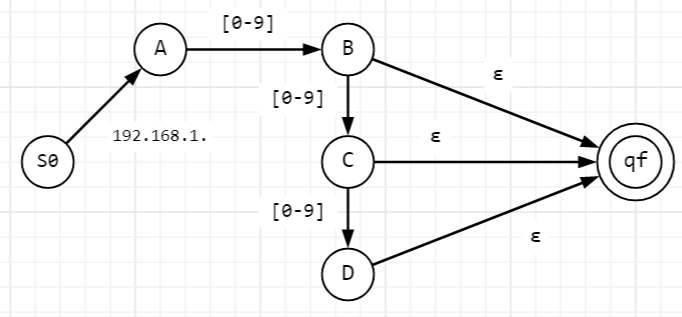
\includegraphics[scale=0.7]{ka_diagram.png}
		Рисунок 1 - Диаграмма конечного автомата	
	\end{center}
	
	\noindent Листинг программы:
		
	\begin{lstlisting}
var ka1 = new FSAutomate(new List<Symbol>()
	{ "S0", "A", "B", "C", "D", "qf" },
	new List<Symbol>() { "", "0", "1", "2",
		"3", "4", "5", "6", "7", "8", "9",
	"192.168.1." },
	new List<Symbol>() { "qf" },
	"S0");
	
ka1.AddRule("S0", "192.168.1.", "A");
		
for (int i = 0; i < 10; i++)
	ka1.AddRule("A", i.ToString(), "B");
		
for (int i = 0; i < 10; i++)
	ka1.AddRule("B", i.ToString(), "C");
	ka1.AddRule("B", "", "qf");
		
	for (int i = 0; i < 10; i++)
	ka1.AddRule("C", i.ToString(), "D");
	ka1.AddRule("C", "", "qf");
	ka1.AddRule("D", "", "qf");
	\end{lstlisting}
	
	\section{Практическая работа №2}
	
	Заданная грамматика:
	
	\begin{gather*}
		G = \{(a, b, c, d, f, \varepsilon, z, r, t, g), \\
			(S, A, B, C, D, R, T, H, G, V), \\
			(A \rightarrow bC, \\
			 B \rightarrow cA, \\
			 C \rightarrow dB, \\
			 D \rightarrow R, \\
			 R \rightarrow f, \\
			 S \rightarrow aABT, \\ 
			 T \rightarrow \varepsilon, \\ 
			 H \rightarrow z, \\
			 G \rightarrow r, \\ 
			 S \rightarrow gV, \\ 
			 V \rightarrow Vt, \\ 
			 V \rightarrow t \\
			S \}
	\end{gather*}
	
	\subsection{Устранение $\varepsilon$-правил, бесполезных символов и цепных правил из грамматики}
	
	В данном случае очевидно, что $\varepsilon$-правило имеет вид $T \rightarrow \varepsilon$, удалим его.
	Получилось так, что нетерминал $T$ стал непроизводящим, удалим его из правой части правила $S \rightarrow aABT$ и получим $S \rightarrow aAB$. Также зметим наличие цепного правила 
	
	\begin{gather*}
		D \rightarrow R, \\
		R \rightarrow f	
	\end{gather*}
	
	Преобразуем эти правила следующим образом:
	
	\begin{gather*}
		D \rightarrow f
	\end{gather*}
	
	Таким образом, получим следующие правила грамматики:
	
	\begin{gather*}
		A \rightarrow bC, \\
		B \rightarrow cA, \\
		C \rightarrow dB, \\
		D \rightarrow f, \\
		S \rightarrow aAB, \\  
		S \rightarrow gV. \\
		V \rightarrow t, \\ 
		V \rightarrow tV', \\
		V' \rightarrow t, \\
		V' \rightarrow tV'
	\end{gather*}
	
	\subsection{Построение МП-автомата}
	
	\begin{gather*}
		\text{МП} = (Q, \Sigma, \Gamma, \delta, q_0, z_0, F), \\
		Q = \{q\}, \\
		\Sigma = T, \\
		\Gamma = T \cup V. \\
		q_0 = q_0, \\
		z_0 = S_0, \\
		F = {q}. \\
		\delta = \{
		\delta(q, \varepsilon, A) = (q, bC), \\
		\delta(q, \varepsilon, B) = (q, cA), \\
		\delta(q, \varepsilon, C) = (q, dB), \\
		\delta(q, \varepsilon, D) = (q, f), \\
		\delta(q, \varepsilon, R) = (q, f), \\
		\delta(q_0, \varepsilon, S) = (q, aAB), \\
		\delta(q_0, \varepsilon, S) = (q, gv), \\
		\delta(q, \varepsilon, V) = (q, t), \\
		\delta(q, \varepsilon, V) = (q, tV'), \\
		\delta(q, \varepsilon, V') = (q, t), \\
		\delta(q, \varepsilon, V') = (q, tV;), \\
		\delta(q, a, a) = (q, \varepsilon), \: \forall a \in \Sigma
		\}
	\end{gather*}
	
	\subsection{Реализация МП-автомата}
	
	\begin{lstlisting}
var regGr = new Grammar(new List<Symbol>() { "a", "b", "c", "d", "f", "t", "g", "z", "r" },
new List<Symbol>() { "S", "A", "B", "C", "D", "R", "T", "V", "H", "G" },
"S");
regGr.AddRule("A", new List<Symbol>() { "b", "C"});
regGr.AddRule("B", new List<Symbol>() { "c", "A" });
regGr.AddRule("C", new List<Symbol>(RST$ & $M$ \\) { "d", "D" });
regGr.AddRule("D", new List<Symbol>() { "R" });
regGr.AddRule("R", new List<Symbol>() { "f" });
regGr.AddRule("S", new List<Symbol>() { "a", "A", "B", "T" });
regGr.AddRule("T", new List<Symbol>() { "" });
regGr.AddRule("H", new List<Symbol>() { "z" });
regGr.AddRule("G", new List<Symbol>() { "r" });
regGr.AddRule("S", new List<Symbol>() { "g", "V" });
regGr.AddRule("V", new List<Symbol>() { "V", "t" });
regGr.AddRule("V", new List<Symbol>() { "t" });

Console.WriteLine("Grammar:");
regGr.Debug("T", regGr.T);
regGr.Debug("T", regGr.V);
regGr.DebugPrules();
Grammar G1 = regGr.EpsDelete();
G1.DebugPrules();
Grammar G2 = G1.unUsefulDelete();
G2.DebugPrules();
Grammar G3 = G2.ChainRuleDelete();
G3.DebugPrules();
Grammar G4 = G3.LeftRecursDelete_new6();
G4.DebugPrules();
// G4 - приведенная грамматика
Console.WriteLine("--------------------------------------------");
Console.WriteLine("Normal Grammatic:");
G4.Debug("T", G4.T);
G4.Debug("V", G4.V);
G4.DebugPrules();
Console.Write("Start symbol: ");
Console.WriteLine(G4.S0 + "\n");		
	\end{lstlisting}	
	
	\section{Построение $LL(K)$-анализатора}
	
	КС-грамматика $G = (T, V, P, S)$ без $\varepsilon$-правил называется простой $LL(1)$ грамматикой ($s$-
	грамматикой, разделенной грамматикой), если для каждого $v \in V$ все его альтернативы начинаются различными терминальными символами. Единица в названии алгоритма означает, что при чтении
	анализируемой цепочки, находящейся на входной ленте, входная головка может заглядывать вперед на
	один символ.
	
	\subsection{Удаление правого ветвоения из грамматики}
	
	Применив алгоритм факторизации для устранения правого ветвления к исходной грамматике, получим следующий набор правил:
	
	\begin{gather*}
		A \rightarrow bC, \\
		B \rightarrow cA, \\
		C \rightarrow dB, \\
		D \rightarrow f, \\
		S \rightarrow aAB, \\  
		S \rightarrow gV. \\
		V \rightarrow tT, \\ 
		V' \rightarrow tT', \\
		T \rightarrow V', \\
		T \rightarrow \varepsilon
	\end{gather*}	
	
	Приведём аналитическое представление управляющей таблицы $M$:
	
	\begin{center}
		
	Таблица 1 - Управляющая таблица анализатора
	
	\begin{tabular}{| c | c | c |}
		\hline
		$A \rightarrow bC$ & $FIRST(A) = b$ & $M(A, b) = (bC, 1)$ \\
		\hline
		$B \rightarrow cA$ & $FIRST(B) = c$ & $M(B, c) = (cA, 2)$ \\
		\hline
		$C \rightarrow dB$ & $FIRST(C) = d$ & $M(C, d) = (db, 3)$ \\
		\hline
		$D \rightarrow f$ & $FIRST(D) = d$ & $M(D, f) = (f, 4)$ \\
		\hline
		$S \rightarrow aAB$ & $FIRST(S) = a$ & $M(S, a) = (aAb, 5)$ \\  
		\hline
		$S \rightarrow gV$ & $FIRST(S) = g$ & $M(S, g) = (V, 7)$ \\
		\hline
		$V \rightarrow tT$ & $FIRST(V) = g$ & $M(V, t) = (tT, 8)$ \\ 
		\hline
		$V' \rightarrow tT'$ & $FIRST(V) = t$ & $M(V', t) = (tT, 9)$ \\
		\hline
		$T \rightarrow V'$ & $FIRST(T) = t$ & $M(T, t) = (V', 10)$ \\
		\hline
		$T \rightarrow \varepsilon$  & $FIRST(T) = \varepsilon$ & $M(T, \varepsilon) = (\varepsilon, 11)$ \\
		\hline
	\end{tabular}
	
	\end{center}
	
	\subsection{Реализация LL(K)-анализатора}
	
	\begin{lstlisting}[language=C]
var LL = new Grammar(new List<Symbol>() 
{ "a", "b", "c", "d", "f", "t", "g", " " },
new List<Symbol>()
{ "S", "A", "B", "C", "D", "R", "V", "V'", "T" },
"S");
LL.AddRule("A", new List<Symbol>() { "b", "C" });
LL.AddRule("B", new List<Symbol>() { "c", "A" });
LL.AddRule("C", new List<Symbol>() { "d", "D" });

LL.AddRule("D", new List<Symbol>() { "f" });
LL.AddRule("R", new List<Symbol>() { "f" });
LL.AddRule("S", new List<Symbol>() { "a", "A", "B" });
LL.AddRule("S", new List<Symbol>() { "g", "V" });
LL.AddRule("V", new List<Symbol>() { "t", "T" });
LL.AddRule("V'", new List<Symbol>() { "t", "T" });
LL.AddRule("T", new List<Symbol>() { "V'" });
LL.AddRule("T", new List<Symbol>() { " " });
var parser = new LLParser(LL);
Console.WriteLine("Введите строку: ");
string stringChain = Console.ReadLine();
var chain = new List<Symbol> { };
foreach (var x in stringChain)
chain.Add(new Symbol(x.ToString()));
if (parser.Parse(chain))
{
	Console.WriteLine("Допуск. Цепочка символов = L(G).");
	Console.WriteLine(parser.OutputConfigure);
}
else
{
	Console.WriteLine("Не допуск. Цепочка символов не = L(G).");
}
	\end{lstlisting}
	
\end{document}